\documentclass[11pt,a4paper]{article}
\usepackage[a4paper,margin=2.4cm]{geometry}
\usepackage[utf8]{inputenc}
\usepackage[T1]{fontenc}
\usepackage[spanish,es-tabla]{babel}
\usepackage{amsmath,amssymb,booktabs,graphicx,float,tabularx,enumitem}
\usepackage[dvipsnames]{xcolor}
\usepackage{hyperref}
\graphicspath{{Fig/}}
\hypersetup{colorlinks=true,linkcolor=MidnightBlue,urlcolor=MidnightBlue,
  pdftitle={Elementos difractivos y deconvoluci\'on},pdfauthor={Francisco Alfaro Medina}}
\setlength{\parindent}{0pt}
\setlength{\parskip}{0.55em}
\setlength{\emergencystretch}{3em}
\renewcommand{\arraystretch}{1.12}
\title{\large Universidad T\'ecnica Federico Santa Mar\'ia\\Departamento de Inform\'atica\\[0.5em]
\rule{\linewidth}{0.5pt}\\[0.4em]\LARGE\textbf{Elementos difractivos y deconvoluci\'on}\\
\large Tarea 4 -- Fotograf\'ia Computacional (INF-449)\\[-0.2em]\rule{\linewidth}{1.2pt}}
\author{Francisco Alfaro Medina}
\date{Octubre de 2026}
\begin{document}
\maketitle

\begin{abstract}
Se implementa en Python un sistema RGB con elemento \'optico difractivo, sensor Bayer RGGB y reconstrucci\'on. La PSF se calcula a partir de una pupila circular con fase c\'ubica y seis modos de Zernike. Se comparan Wiener y Richardson--Lucy implementados desde cero con `skimage.restoration`, y adem\'as se resuelve la regularizaci\'on de la ecuaci\'on (2) directamente sobre la medici\'on Bayer mediante gradiente conjugado. La evaluaci\'on usa las 18 im\'agenes McMaster disponibles en \texttt{tareas/tarea-04/McMaster}, a $256\times256$ p\'ixeles, sin ruido aditivo en el experimento principal. Wiener constante mejora el PSNR medio de 16.48 a 22.72 dB y SSIM de 0.3778 a 0.6724; Richardson--Lucy logra 21.27 dB y 0.5798. La regularizaci\'on Laplaciana de referencia de \texttt{skimage} obtiene el mayor promedio (24.29 dB, 0.7431), aunque usa un prior distinto al Wiener de la ecuaci\'on (4). Las FFT propias de PSF y Wiener se ejecutaron en una NVIDIA RTX 4060 Laptop mediante CUDA.
\end{abstract}

\section{Enunciado y fuentes}
La gu\'ia solicita (i) modelar un sistema difractivo RGB con fase c\'ubica y modos de Zernike, (ii) usar las 18 im\'agenes McMaster, (iii) implementar Wiener y Richardson--Lucy desde cero y contrastarlos con \texttt{skimage.restoration}, y (iv) graficar PSNR, SSIM y SAM sobre el dataset. Las ecuaciones (1)--(10) y estas m\'etricas se toman de \texttt{tareas/tarea-04/homework4.pdf}, pp. 1--4.

La notaci\'on \'optica sigue \texttt{files/lecture4a.pdf}, diapositivas 7--11 (modelo difractivo y Zernike de Noll), y \texttt{files/lecture4b.pdf}, diapositivas 6 y 13 (fase c\'ubica y desenfoque) \cite{lecture4a,lecture4b}. El libro de David J. Brady, \emph{Computational Optical Imaging}, cap. 2, sec. 2.6, p. 52, respalda el modelo directo discreto; cap. 3, sec. 3.2, p. 96, los sistemas invariantes al desplazamiento y su respuesta en frecuencia; cap. 5, sec. 5.3, p. 196, la formaci\'on por difracci\'on \cite{brady}. La gu\'ia aporta las ecuaciones espec\'ificas de Wiener y Richardson--Lucy. El material \texttt{extra/material\_curso/homework4/} contiene las bandas Washington DC y el c\'odigo MATLAB de Zernike, cuya base de Noll se port\'o a Python. Se revisaron tambi\'en \texttt{Chapter3ImageEstimation/wienerFiltering.ipynb} y \texttt{Chapter5WaveImaging/numericalDiffraction.ipynb} como ejemplos de estos conceptos.

\section{Modelo y m\'etodo}
\subsection{Elemento difractivo y PSF}
Sean $x,y$ coordenadas normalizadas dentro de una pupila circular $A(x,y)=\mathbf{1}_{x^2+y^2\leq1}$, $\rho=\sqrt{x^2+y^2}$ y $\theta=\operatorname{atan2}(y,x)$. A $\lambda_0=550$ nm, la fase aplicada es
\begin{equation}
\phi(x,y)=A(x,y)\left[6\pi(x^3+y^3)+\sum_{j\in\{4,5,6,7,8,11\}}a_jZ_j(\rho,\theta)\right],
\end{equation}
con $[a_4,a_5,a_6,a_7,a_8,a_{11}]=[0.6,0.4,-0.3,0.3,-0.2,0.3]$ rad. Los $Z_j$ usan la normalizaci\'on de Noll implementada en el c\'odigo. Para cada canal se escala la fase por $\lambda_0/\lambda$, se calcula $h_\lambda=|\mathcal{F}\{A\exp(i\lambda_0\phi/\lambda)\}|^2$ y se normaliza la PSF recortada a $161\times161$ a suma unitaria. El FFT de la pupila usa una grilla $256\times256$ con muestreo que evita aliasing del soporte de la PSF en la configuraci\'on elegida.
La apertura libre sirve como referencia para cuantificar el costo de codificar el frente de onda. En el canal verde, la PSF del DOE combinado tiene ancho RMS de 17.51 px y MTF de 0.0308 a 0.25 ciclos/px; la apertura libre da 7.11 px y 0.2752. El DOE distribuye la energ\'ia en una PSF m\'as amplia y aten\'ua las frecuencias altas, por lo que la reconstrucci\'on inversa requiere regularizaci\'on.
\begin{table}[H]\centering\small
\caption{Diagn\'osticos de PSF del canal verde (550 nm), desde \texttt{resultados/psf\_diagnosticos.csv}.}
\label{tab:mtf}\begin{tabular}{lccc}\toprule
Dise\~no & Energ\'ia en ventana & Ancho RMS [px] & MTF a 0.25 ciclos/px \tabularnewline\midrule
Apertura libre & 0.9956 & 7.11 & 0.2752 \tabularnewline
C\'ubica + Zernike & 0.9937 & 17.51 & 0.0308 \tabularnewline\bottomrule\end{tabular}\end{table}
\begin{figure}[H]\centering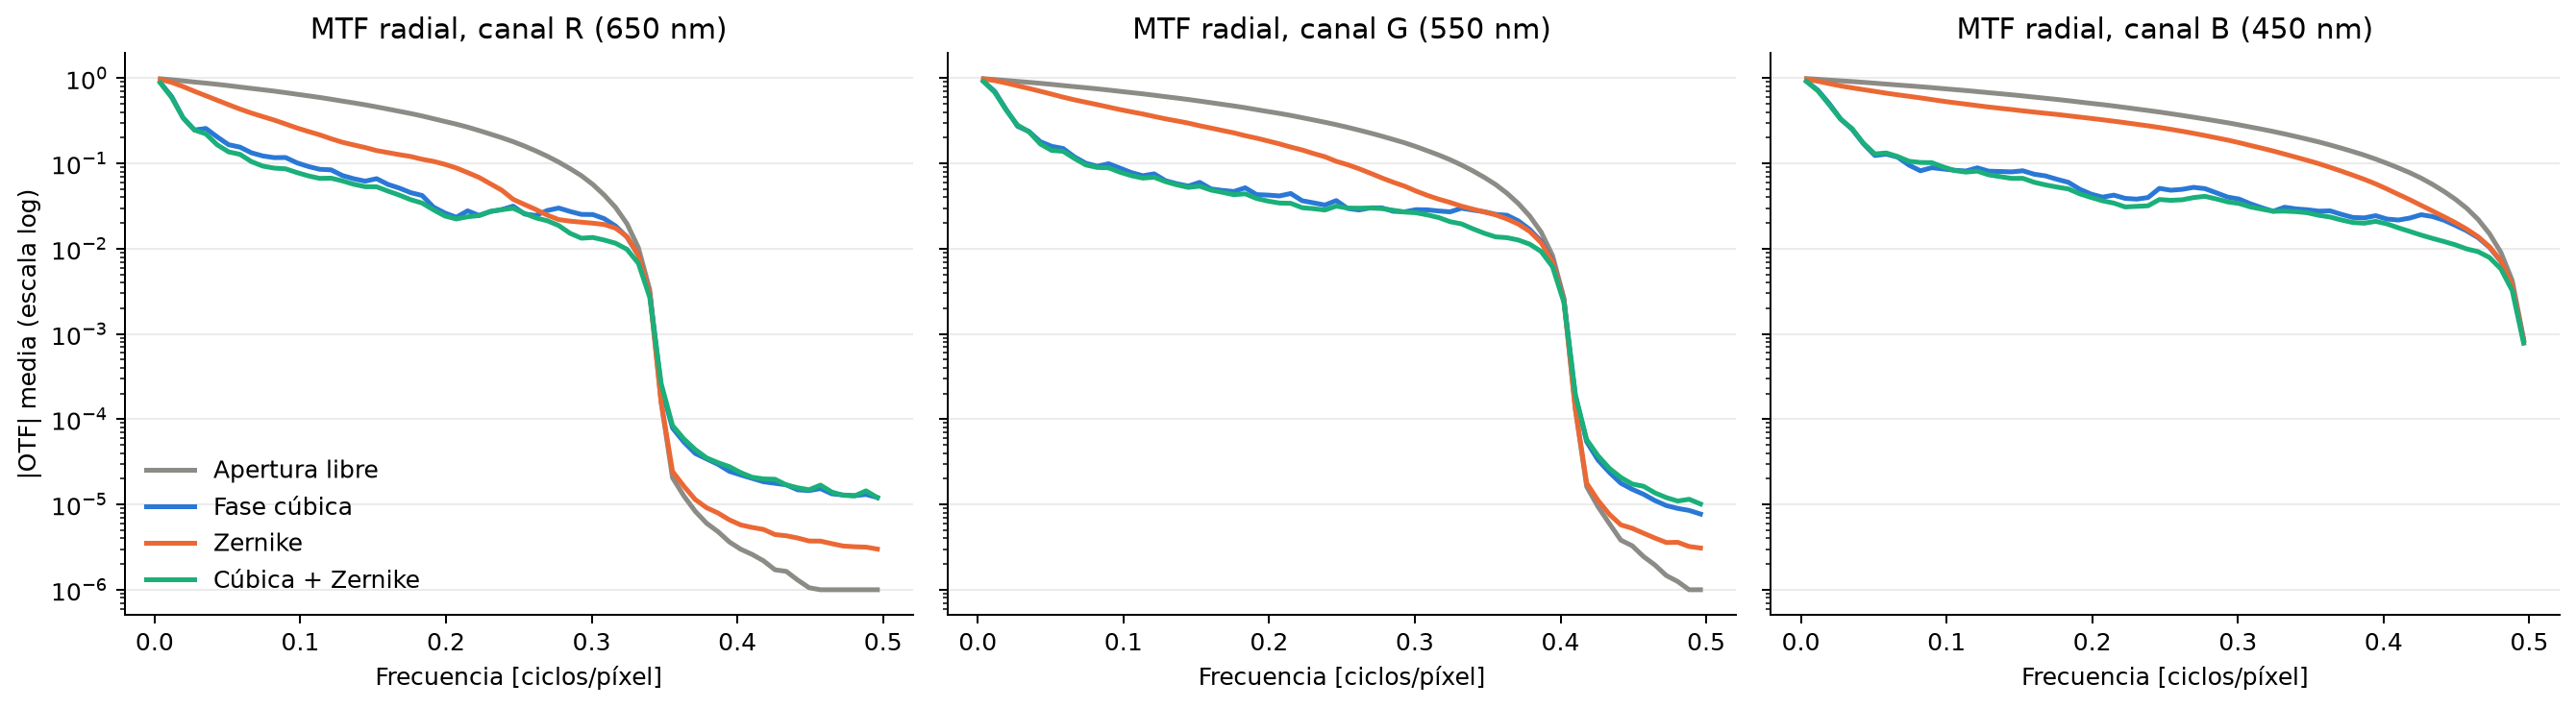
\includegraphics[width=0.9\linewidth]{mtf_disenos.png}
\caption{MTF radial por canal para apertura libre y los disenos DOE. La caida espectral explica por que la inversion amplifica errores si $|H_c|$ se aproxima a cero.}\label{fig:mtf}\end{figure}

\begin{figure}[H]\centering
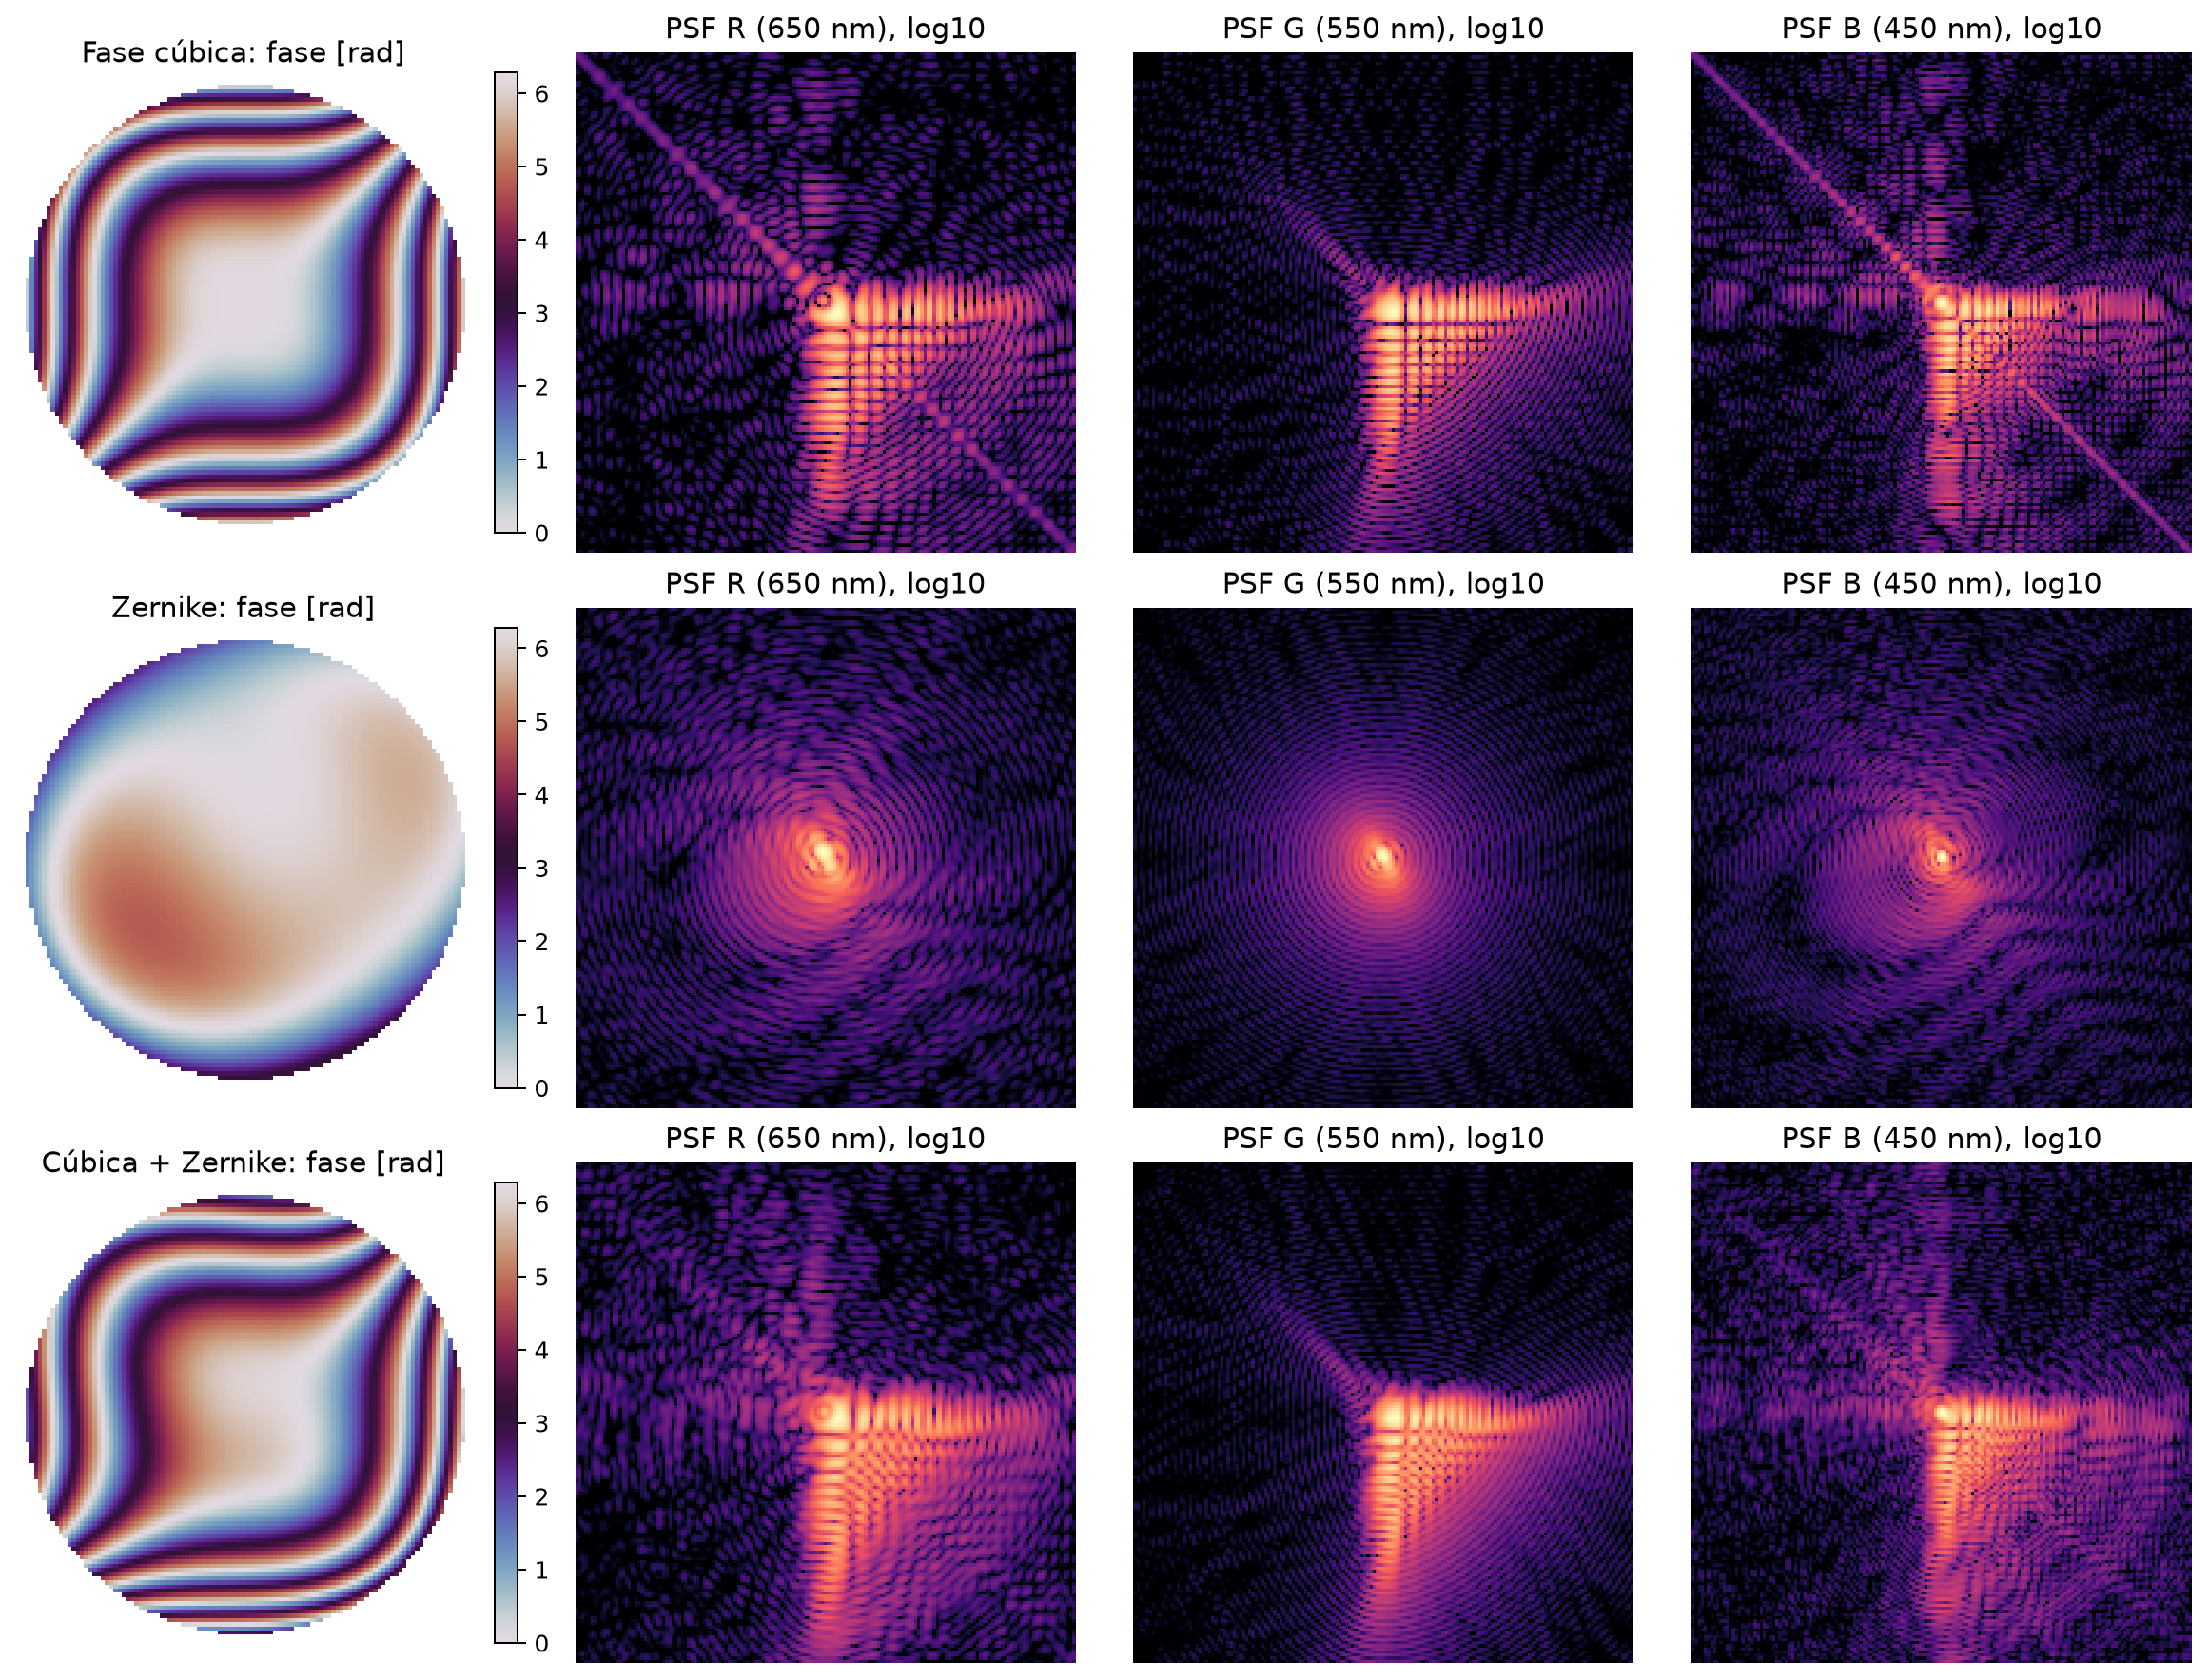
\includegraphics[width=0.94\linewidth]{psf_doe.png}
\caption{Fase envuelta y PSF para los tres canales espectrales del dise\~no combinado. La intensidad se muestra en escala logar\'itmica.}
\label{fig:psf}\end{figure}

\subsection{Sensor y reconstrucci\'on}
Cada canal se convoluciona con su PSF usando extensi\'on sim\'etrica en los bordes. El mosaico Bayer RGGB conserva una muestra por p\'ixel; el demosaicking bilineal interpola cada color y reimpone las muestras observadas. El experimento principal no agrega ruido ($\sigma=0$). Las im\'agenes originales de $500\times500$ se redimensionan a $256\times256$ con Lanczos y se normalizan a $[0,1]$.

Se implementa el filtro de Wiener
\begin{equation}
\widehat I_c=\mathcal{F}^{-1}\!\left\{\frac{H_c^*}{|H_c|^2+\tau}\,\mathcal{F}\{\widetilde I_c\}\right\},\qquad \tau=0.01,
\end{equation}
con extensi\'on sim\'etrica antes de la FFT y recorte al tama\~no de la imagen despu\'es. La estimaci\'on de $\tau$ de la ecuaci\'on (5) se reporta como diagn\'ostico; su cociente global no necesariamente representa la distribuci\'on espectral del error de interpolaci\'on. En un sistema invariante al desplazamiento, el filtro actua frecuencia por frecuencia: el termino $|H_c|^2+\tau$ evita la division inestable por una OTF pequena, como se discute en el cap. 3, sec. 3.2.

Richardson--Lucy usa la actualizaci\'on multiplicativa de la ecuaci\'on (6), $K=25$ iteraciones y una inicializaci\'on constante positiva de 0.5. Para comparar justamente con \texttt{skimage}, se usan la misma medici\'on demosaickeada, PSF, regularizaci\'on/iteraciones y rango final $[0,1]$. En Wiener se incluye la opci\'on por defecto de \texttt{skimage} con regularizador Laplaciano como referencia adicional; esta variante no corresponde al prior constante de la ecuaci\'on (4).

Tambi\'en se resuelve el problema regularizado de la ecuaci\'on (2) sobre el mosaico Bayer, sin demosaicking previo, mediante gradiente conjugado y regularizaci\'on $\tau_{\rm Bayer}=10^{-3}$. Esta extensi\'on permite contrastar la cadena demosaicking-m\'as-deconvoluci\'on con una estimaci\'on directa desde la medici\'on.

\begin{figure}[H]\centering
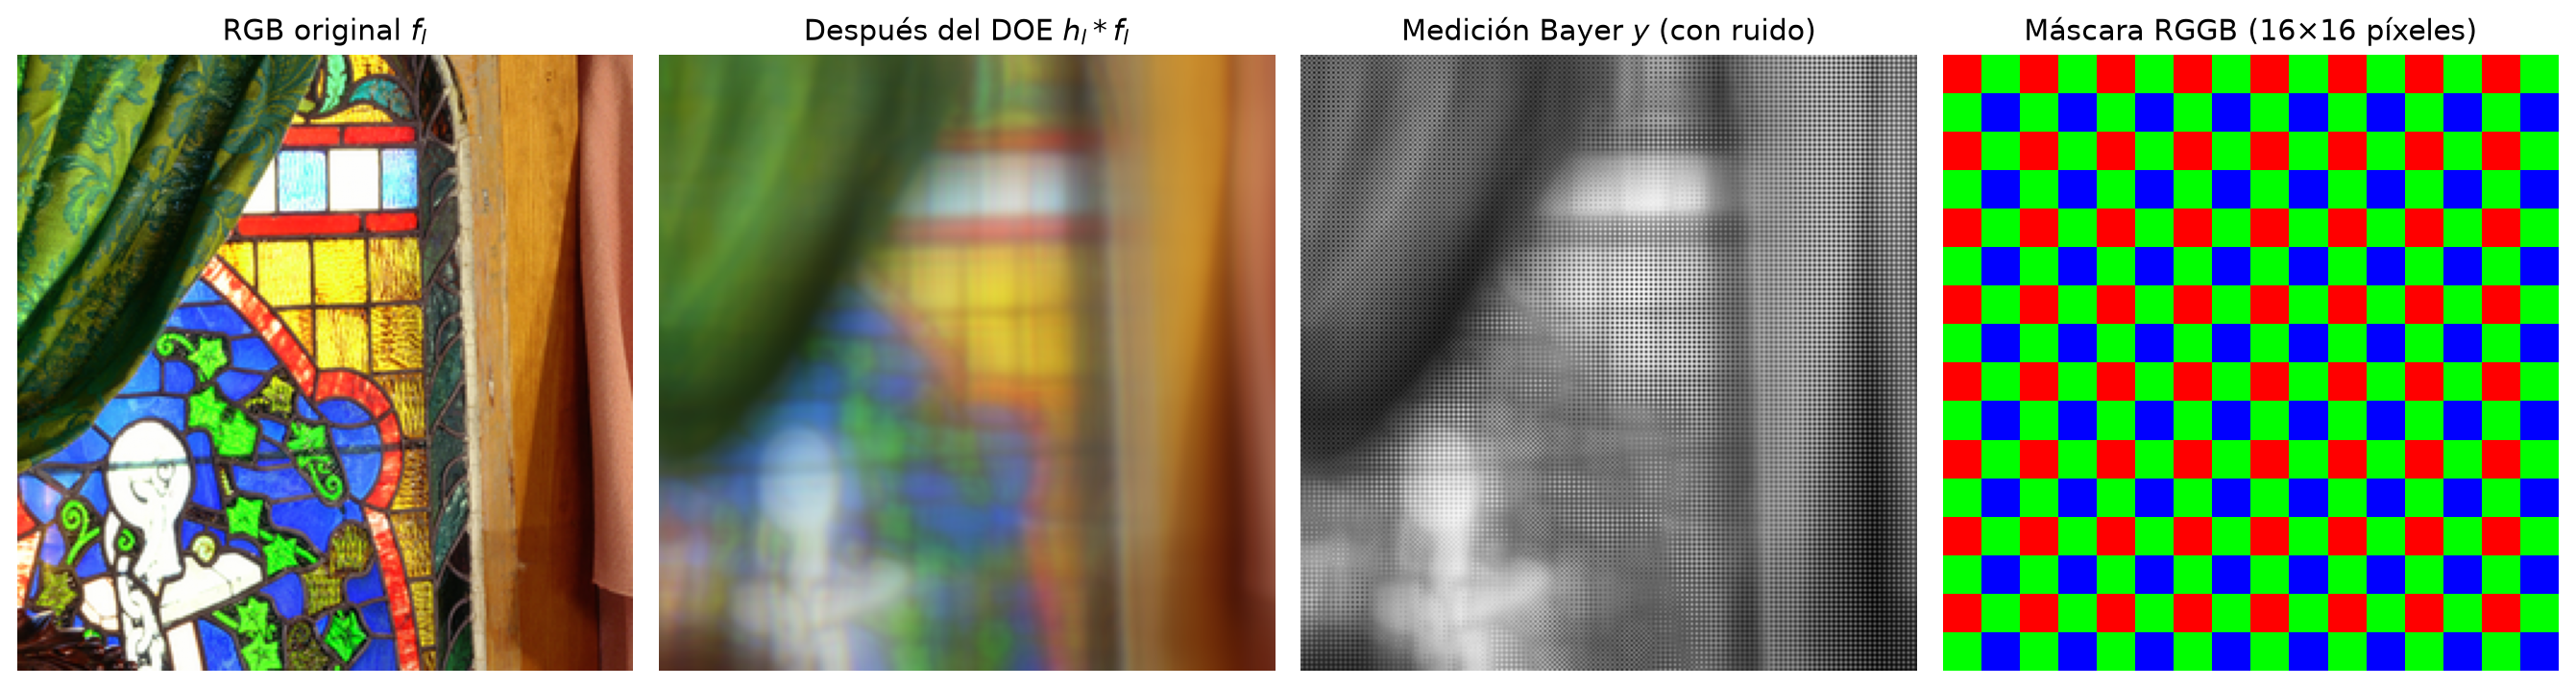
\includegraphics[width=\linewidth]{modelo_sensor.png}
\caption{Imagen McMaster 1, canales desenfocados, medici\'on Bayer y patr\'on RGGB.}
\label{fig:sensor}\end{figure}

\subsection{M\'etricas y c\'alculo}
Para dos RGB de referencia $I$ y reconstruccion $\widehat I$, PSNR usa el MSE conjunto de los tres canales y rango dinamico 1:
\begin{equation}
\operatorname{MSE}=\frac{1}{3HW}\sum_{i,j,c}(I_{ijc}-\widehat I_{ijc})^2,\qquad \operatorname{PSNR}=10\log_{10}\!\left(\frac{1}{\operatorname{MSE}}\right).
\end{equation}
SSIM se calcula por canal con ventana uniforme $7\times7$, $K_1=0.01$, $K_2=0.03$, $C_1=K_1^2$ y $C_2=K_2^2$, y luego se promedia:
\begin{equation}
\operatorname{SSIM}(x,y)=\frac{(2\mu_x\mu_y+C_1)(2\sigma_{xy}+C_2)}{(\mu_x^2+\mu_y^2+C_1)(\sigma_x^2+\sigma_y^2+C_2)}.
\end{equation}
SAM es el angulo espectral medio entre los vectores RGB en cada pixel, convertido a grados; si ambos vectores son negros se define como cero:
\begin{equation}
\operatorname{SAM}=\frac{180}{\pi HW}\sum_{i,j}\arccos\!\left(\frac{I_{ij}\cdot\widehat I_{ij}}{\|I_{ij}\|_2\,\|\widehat I_{ij}\|_2}\right).
\end{equation}
\section{Resultados}
\subsection{Promedio sobre McMaster}
La Tabla~\ref{tab:promedios} muestra media y desviaci\'on est\'andar poblacional por imagen. Las m\'etricas por imagen y las figuras se generan desde el mismo CSV. El demosaicking es la l\'inea base; las implementaciones propias de Wiener y RL coinciden con sus referencias de \texttt{skimage} al usar la misma formulaci\'on. El regularizador Laplaciano y Tikhonov Bayer se incluyen como comparadores complementarios.

\begin{table}[H]\centering\small
\caption{Media $\pm$ desviaci\'on est\'andar poblacional en 18 im\'agenes McMaster.}
\label{tab:promedios}\begin{tabular}{lccc}
\toprule
Método & PSNR [dB] & SSIM & SAM [$^\circ$] \\
\midrule
Demosaicking bilineal (sin deconvolución) & $16.48 \pm 2.12$ & $0.3778 \pm 0.1288$ & $9.41 \pm 3.69$ \\
Wiener propio & $22.72 \pm 2.68$ & $0.6724 \pm 0.0909$ & $5.36 \pm 2.33$ \\
Wiener skimage ($\tau$ constante) & $22.72 \pm 2.68$ & $0.6724 \pm 0.0909$ & $5.36 \pm 2.33$ \\
Wiener skimage (Laplaciano, por defecto) & $24.29 \pm 2.78$ & $0.7431 \pm 0.0752$ & $4.83 \pm 2.24$ \\
Richardson--Lucy propio & $21.27 \pm 2.62$ & $0.5798 \pm 0.1141$ & $5.97 \pm 2.43$ \\
Richardson--Lucy skimage & $21.27 \pm 2.62$ & $0.5798 \pm 0.1141$ & $5.97 \pm 2.43$ \\
Ec.~(2) sobre Bayer (Tikhonov, GC) & $22.66 \pm 1.97$ & $0.7290 \pm 0.0580$ & $5.98 \pm 2.53$ \\
\midrule
Demosaicking Malvar (sin deconvolución) & $16.49 \pm 2.13$ & $0.3790 \pm 0.1286$ & $9.41 \pm 3.69$ \\
Malvar + Wiener propio & $22.78 \pm 2.69$ & $0.6734 \pm 0.0910$ & $5.43 \pm 2.39$ \\
\bottomrule
\end{tabular}

\end{table}

\begin{figure}[H]\centering
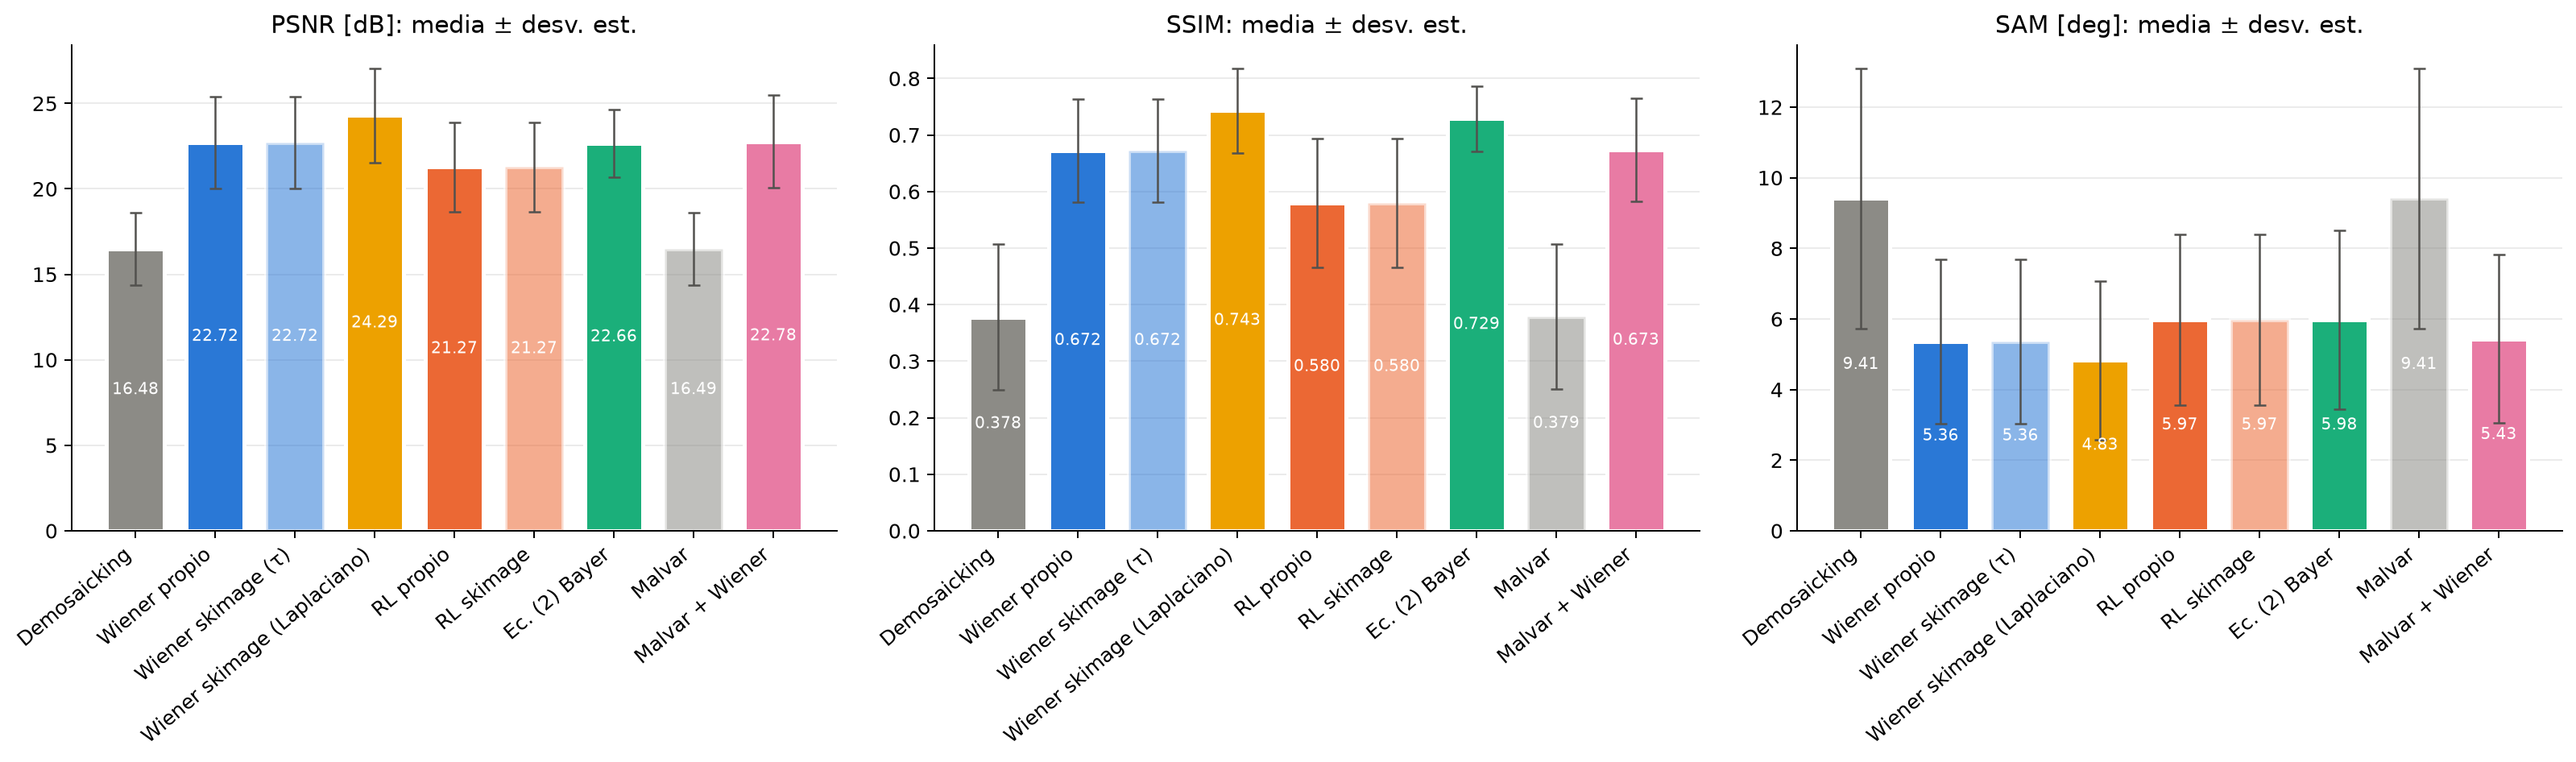
\includegraphics[width=\linewidth]{metricas_dataset.png}
\caption{Media y desviaci\'on est\'andar de PSNR, SSIM y SAM para los m\'etodos de la tabla.}
\label{fig:metricas}\end{figure}

\subsection{Comprobaci\'on de implementaciones}
La Tabla~\ref{tab:comparacion} reporta diferencias m\'aximas entre las implementaciones propias y las referencias. Wiener constante coincide con \texttt{skimage} dentro del redondeo de coma flotante, y RL coincide exactamente en esta configuraci\'on. La diferencia con Wiener Laplaciano es esperable porque la regularizaci\'on dependiente de frecuencia cambia el problema optimizado.
\begin{table}[H]\centering\small
\caption{Diferencia m\'axima entre implementaciones propias y \texttt{skimage} sobre el conjunto.}
\label{tab:comparacion}\begin{tabular}{lcccc}
\toprule
Par comparado & $\max|\Delta \widehat I|$ & $\max|\Delta\mathrm{PSNR}|$ [dB] & $\max|\Delta\mathrm{SSIM}|$ & $\max|\Delta\mathrm{SAM}|$ [$^\circ$] \\
\midrule
Wiener & $4.4\times10^{-15}$ & $3.6\times10^{-15}$ & $2.7\times10^{-14}$ & $1.1\times10^{-14}$ \\
Wiener (vs. Laplaciano) & $0.365$ & $2.235$ & $0.116$ & $1.794$ \\
Richardson--Lucy & $0$ & $0$ & $0$ & $0$ \\
\bottomrule
\end{tabular}

\end{table}

\begin{figure}[H]\centering
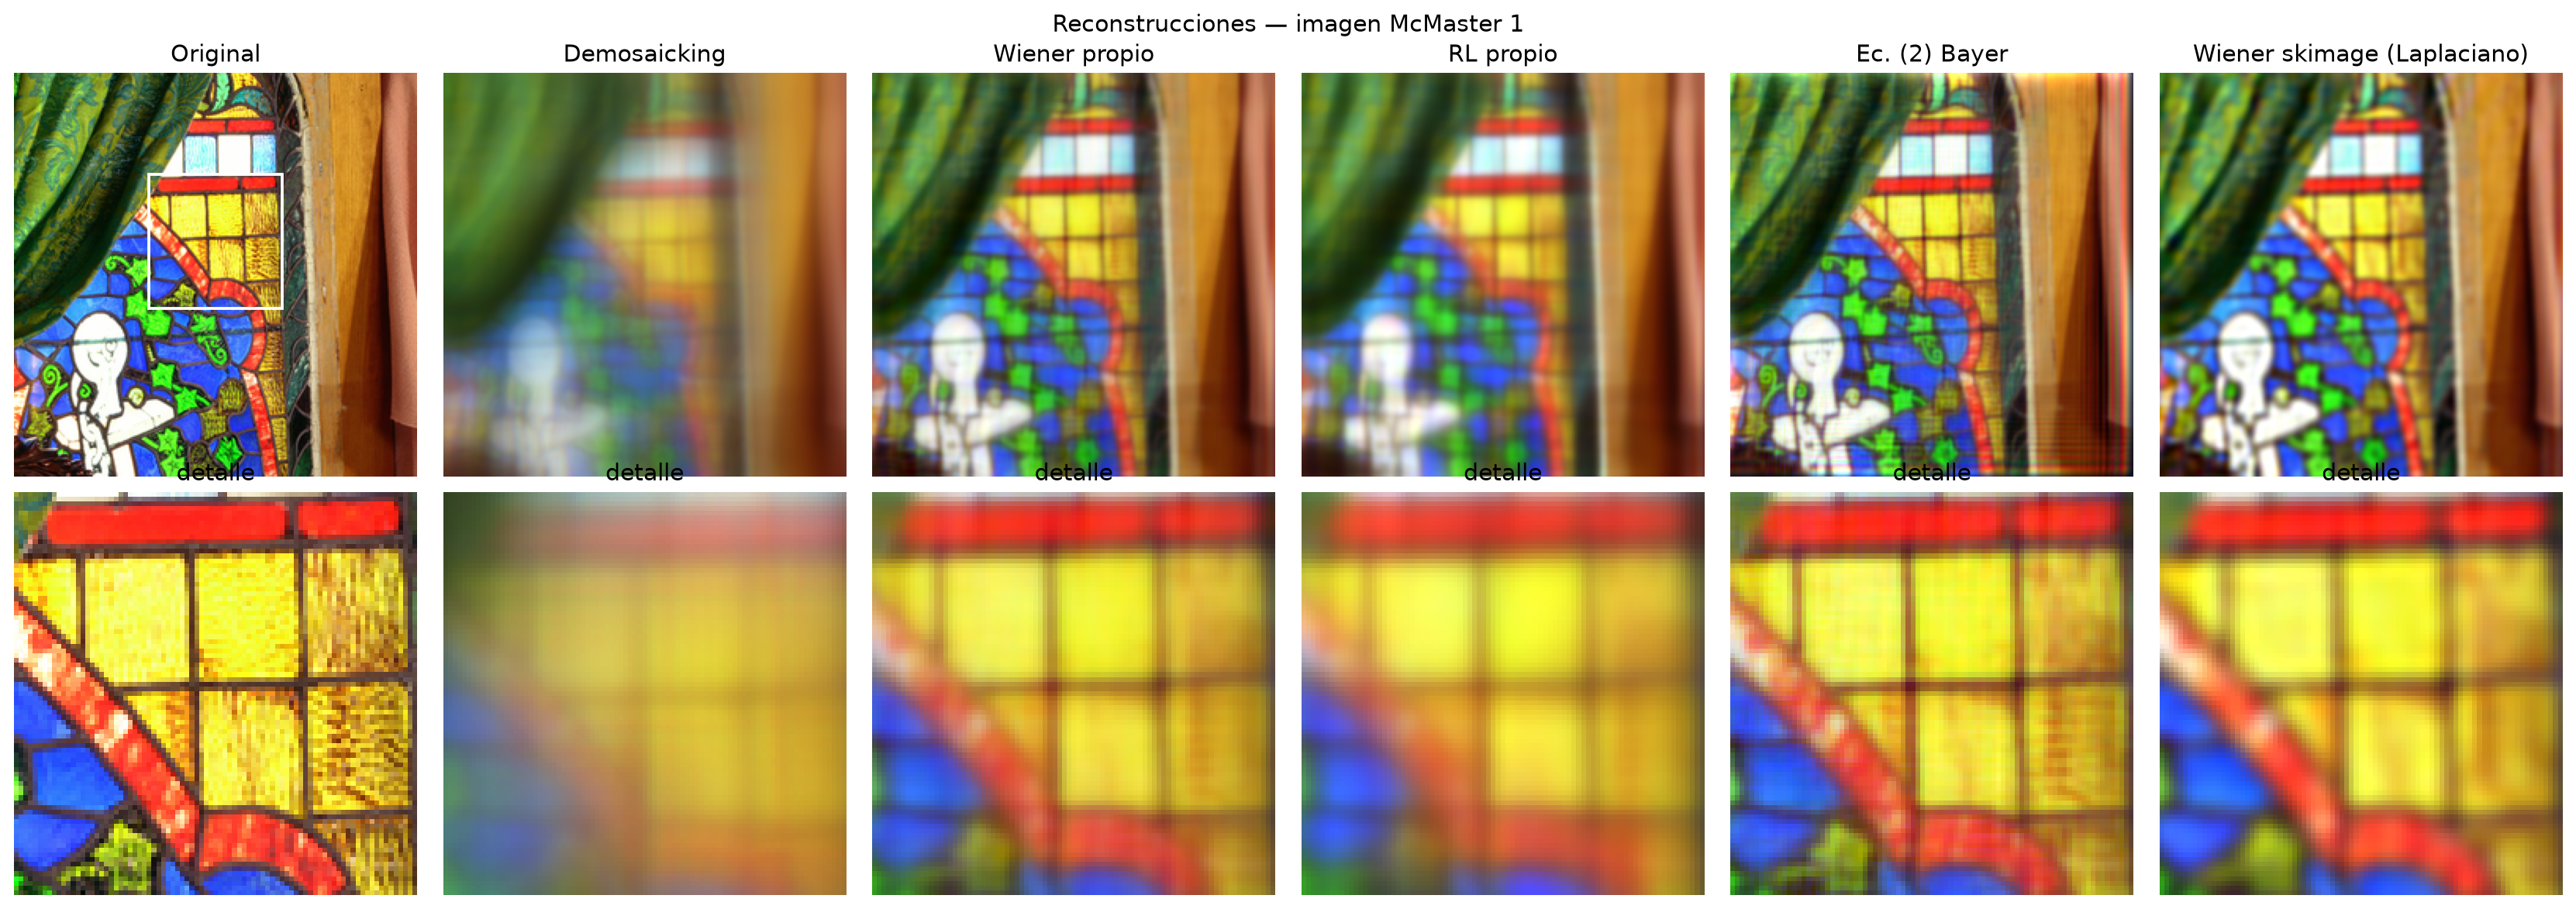
\includegraphics[width=0.98\linewidth]{reconstruccion_ejemplo.png}
\caption{Reconstrucciones de la imagen McMaster 1. Se muestran la imagen original, el demosaicking, Wiener, RL, Tikhonov Bayer y Wiener con regularizaci\'on Laplaciana.}
\label{fig:reconstruccion}\end{figure}

\begin{figure}[H]\centering
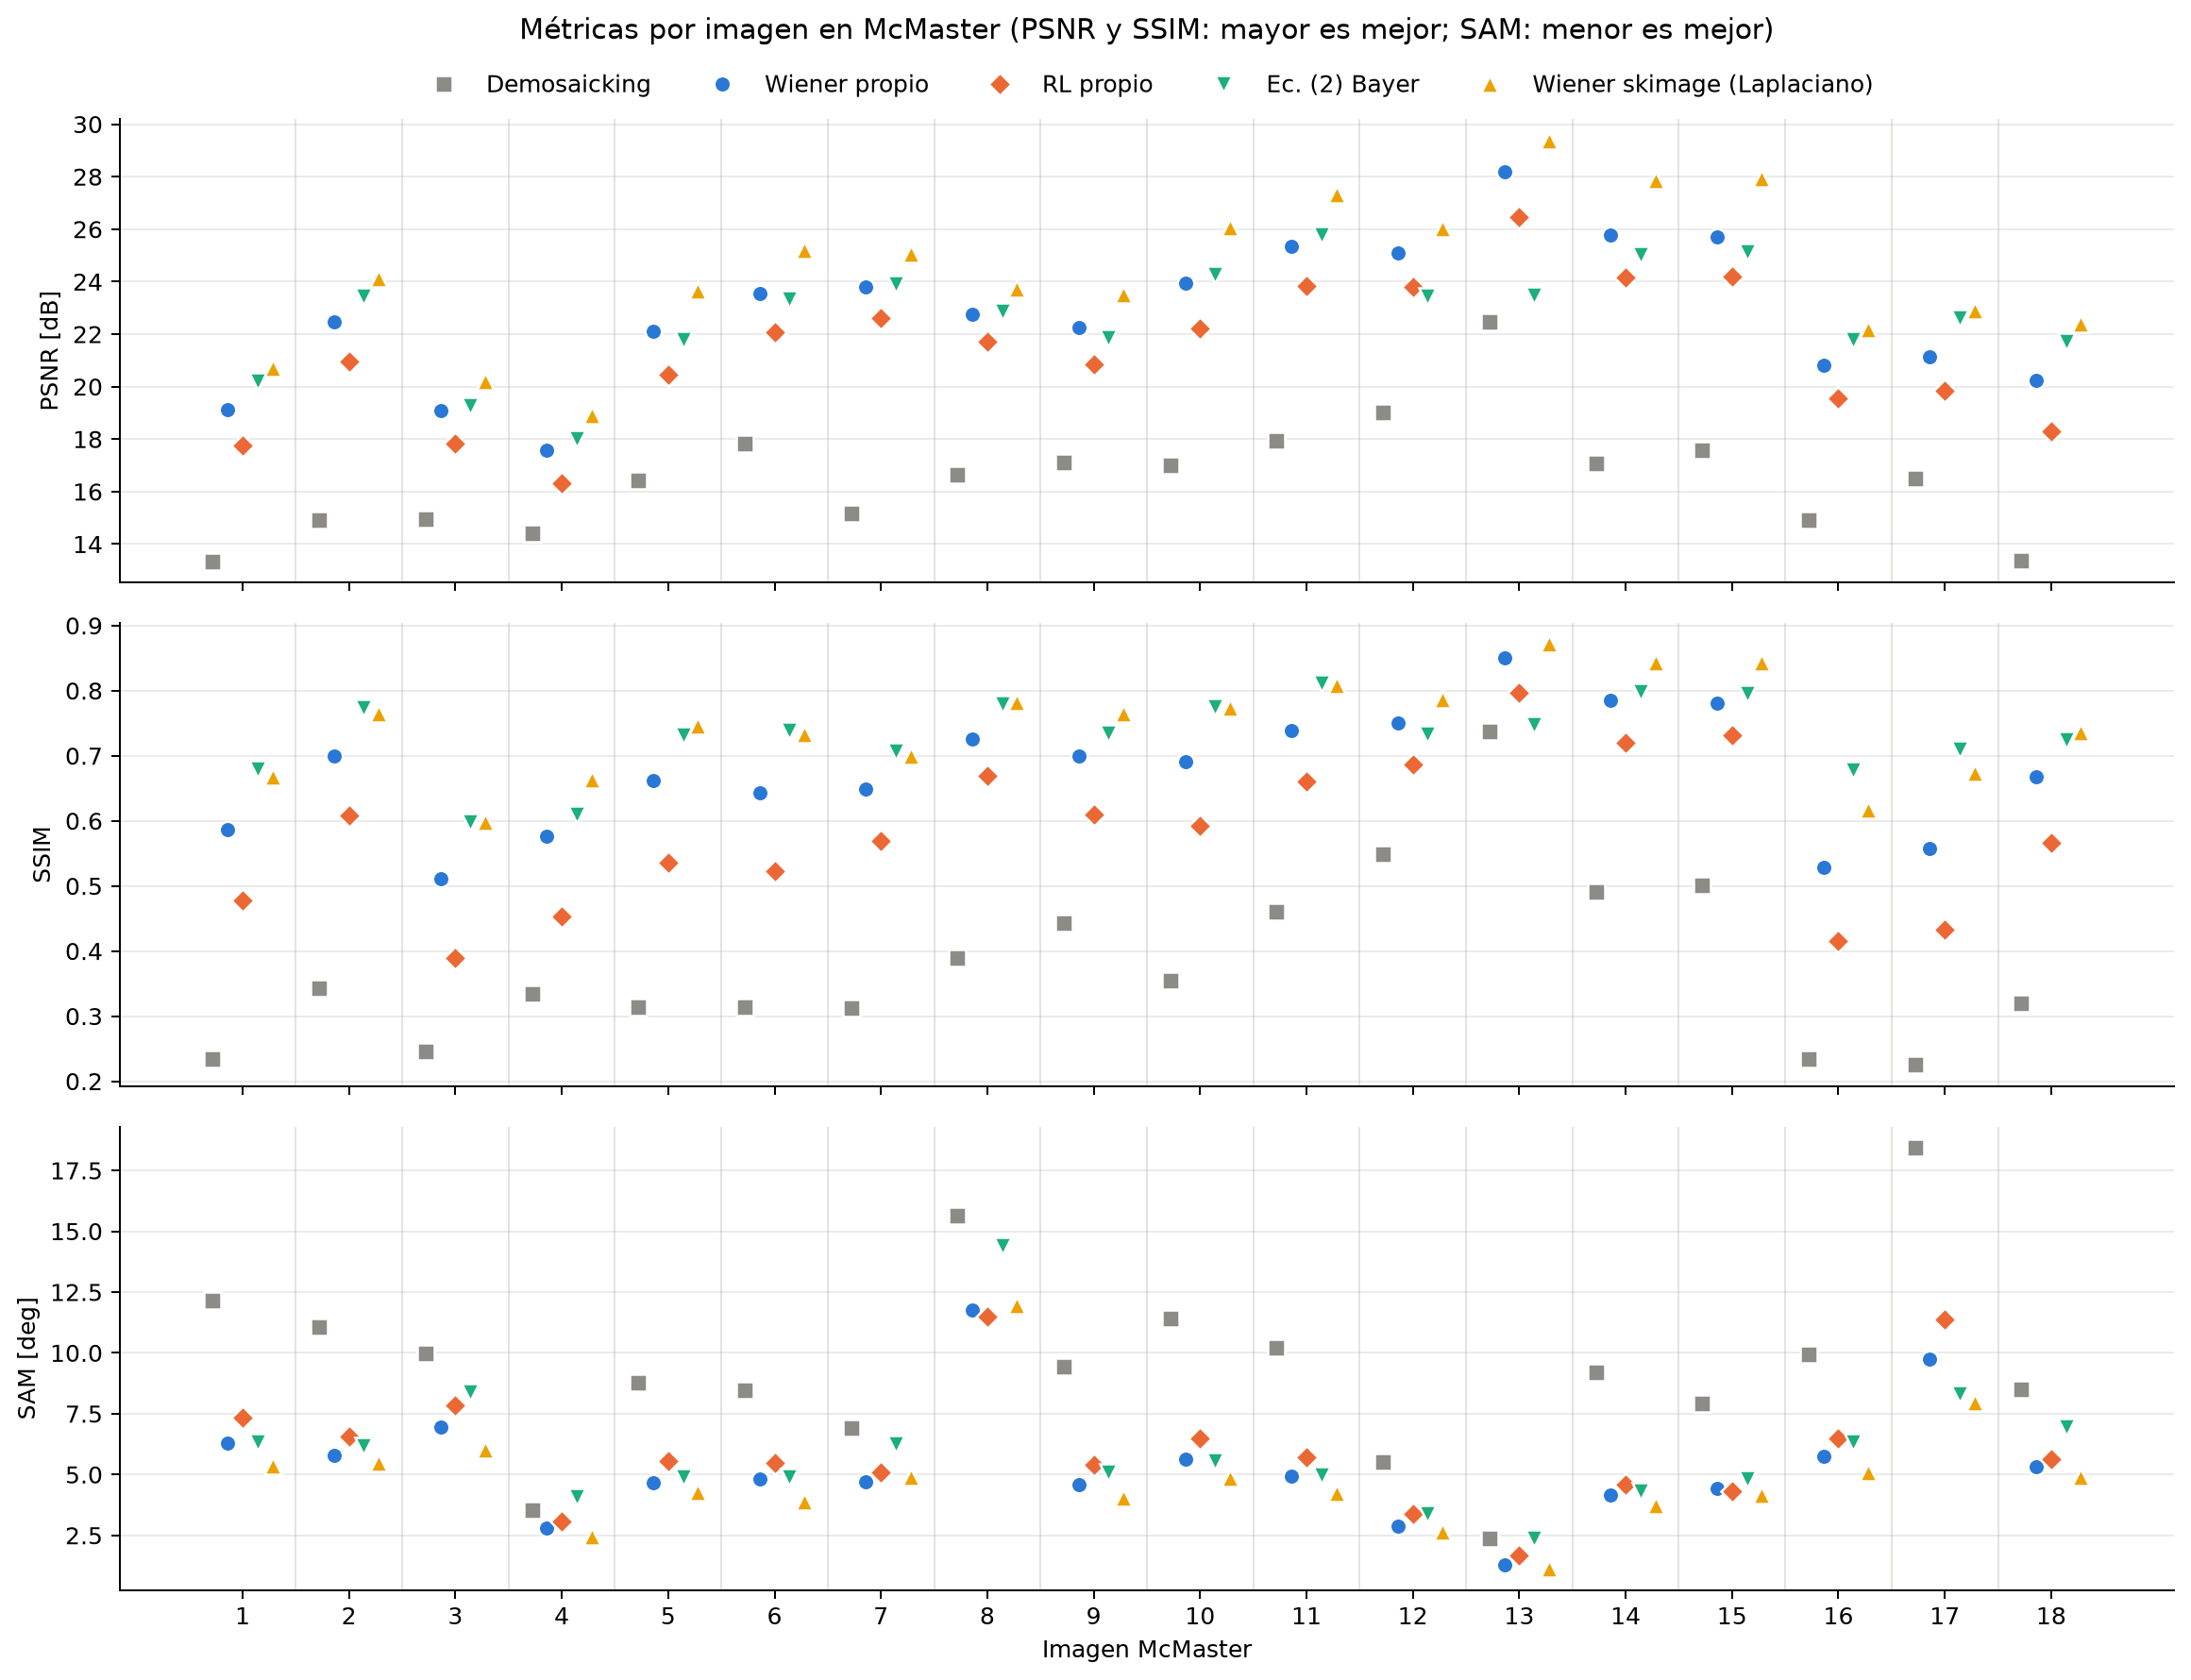
\includegraphics[width=\linewidth]{metricas_por_imagen.png}
\caption{Variaci\'on de las tres m\'etricas entre las 18 im\'agenes.}
\label{fig:porimagen}\end{figure}

\subsection{Lectura de los resultados}
Wiener con $\tau=0.01$ aumenta el PSNR medio en 6.23 dB respecto del demosaicking; RL lo aumenta en 4.79 dB. Wiener Laplaciano logra 24.29 dB y SSIM 0.7431, pero no es comparaci\'on de id\'entico prior. La reconstrucci\'on directa de Bayer alcanza PSNR 22.66 dB y SSIM 0.7290, mostrando que se puede evitar la etapa intermedia de demosaicking al resolver el modelo de sensado. Los promedios de SAM tambi\'on mejoran respecto del demosaicking (9.41$^{\circ}$): 5.36$^{\circ}$ con Wiener constante, 5.97$^{\circ}$ con RL y 5.98$^{\circ}$ con Tikhonov Bayer. Este resultado depende de la PSF, el dise\~no de fase, la escala y el modelo sin ruido; no se extrapola a la resoluci\'on o a condiciones de captura distintas.
En las 18 imagenes, Wiener constante mejora las tres metricas respecto del demosaicking; RL tambien mejora las tres en las 18. Tikhonov directo sobre Bayer mejora PSNR y SSIM en las 18 y SAM en 17. No es solo un cambio en la media: la Tabla~\ref{tab:ganancias} resume diferencias pareadas respecto de la linea base.
\begin{table}[H]\centering\small
\caption{Cambio medio respecto del demosaicking. La \\''ultima columna cuenta im\\'agenes que mejoran simult\\'aneamente PSNR, SSIM y SAM.}
\label{tab:ganancias}\begin{tabular}{lcccc}\toprule
M\\'etodo & $\Delta$PSNR [dB] & $\Delta$SSIM & $\Delta$SAM [$^\circ$] & Mejora conjunta \tabularnewline\midrule
Wiener constante & +6.23 & +0.295 & -4.05 & 18/18 \tabularnewline
Richardson--Lucy & +4.79 & +0.202 & -3.44 & 18/18 \tabularnewline
Tikhonov Bayer & +6.18 & +0.351 & -3.44 & 17/18 \tabularnewline\bottomrule\end{tabular}\end{table}

En terminos practicos, Wiener estandar y Tikhonov Bayer quedan casi empatados en PSNR (22.72 y 22.66 dB), pero Tikhonov obtiene mayor SSIM (0.7290 frente a 0.6724); Wiener conserva mejor el SAM medio (5.36$^\circ$ frente a 5.98$^\circ$). La variante Laplaciana de \texttt{skimage} gana PSNR en las 18 imagenes y SSIM en 10, pero optimiza un prior distinto. El PSNR de Wiener estandar varia de 17.56 dB (imagen 4) a 28.18 dB (imagen 13), lo que muestra dependencia del contenido ademas del metodo.
\begin{table}[H]\centering\small
\caption{Cambio medio respecto del demosaicking. La ultima columna cuenta las imagenes que mejoran simultaneamente PSNR, SSIM y SAM.}
\label{tab:ganancias}\begin{tabular}{lcccc}\toprule
M\'etodo & $\Delta$PSNR [dB] & $\Delta$SSIM & $\Delta$SAM [$^\circ$] & Mejora conjunta \tabularnewline\midrule
Wiener constante & +6.23 & +0.295 & -4.05 & 18/18 \tabularnewline
Richardson--Lucy & +4.79 & +0.202 & -3.44 & 18/18 \tabularnewline
Tikhonov Bayer & +6.18 & +0.351 & -3.44 & 17/18 \tabularnewline\bottomrule\end{tabular}\end{table}


\section{Conclusiones y limitaciones}
\begin{enumerate}[leftmargin=*]
\item Se cubrieron los requerimientos centrales de la gu\'ia: DOE c\'ubico y Zernike, sensor Bayer, reconstrucciones propias de Wiener y Richardson--Lucy, comparaci\'on con \texttt{skimage} y evaluaci\'on PSNR/SSIM/SAM de las 18 im\'agenes McMaster.
\item La deconvoluci\'on mejora la calidad espacial en el promedio del dataset. Entre las variantes propias, Wiener logra mayor PSNR que RL; RL y Wiener optimizan criterios distintos, por lo que se reportan ambas m\'etricas perceptuales.
\item La implementaci\'on de la ecuaci\'on (2) opera directamente sobre el Bayer y obtiene resultados competitivos; su ventaja y color dependen de la regularizaci\'on y del dise\~no \'optico.
\item La PSF es una aproximaci\'on escalar con tres longitudes de onda, sin dispersi\'on del material ni cuantizaci\'on/ruido de fabricaci\'on del DOE. El experimento principal tampoco modela ruido de sensor y reduce las im\'agenes a $256\times256$.
\item CUDA aceler\'o \'unicamente las FFT propias de PSF y Wiener. Los dem\'as pasos siguen en CPU, de modo que el uso de GPU es parcial; el modo `--device cpu` conserva la ruta de respaldo.
\end{enumerate}

El CSV hist\'orico de barrido disponible en la carpeta ten\'ia promedios agregados sin resultados por imagen, por lo que no se mezcl\'o con esta evaluaci\'on ni se us\'o para sustentar conclusiones. Al activar una corrida completa se genera un barrido nuevo con el esquema actual.

\paragraph{Reproducibilidad.} Desde la ra\'iz del repositorio, ejecutar `\.venv/Scripts/python.exe tareas/tarea-04/homework4.py --device auto --workers 2` para rehacer el experimento completo, o `\.venv/Scripts/python.exe tareas/tarea-04/homework4.py --device auto --solo-tablas` para regenerar tablas y gr\'aficos de m\'etricas desde los CSV existentes. El notebook \texttt{homework4.ipynb} carga dichos resultados por defecto y ofrece una variable para lanzar la corrida completa. Las figuras est\'on en \texttt{Fig/}; m\'etricas y diagn\'osticos, en \texttt{resultados/}.

\begin{thebibliography}{9}
\bibitem{guia} N. D\'iaz, \emph{Homework 4: Diffractive Optical Elements and Deconvolution}, INF-449, 1 oct. 2026.
\bibitem{brady} D. J. Brady, \emph{Computational Optical Imaging}, secci\'on 5.3, ``Diffraction'', p. 196.
\bibitem{lecture4a} N. D\'iaz, \emph{Lecture 4a: Diffractive Optical Elements}, diapositivas 7--11, material INF-449.
\bibitem{lecture4b} N. D\'iaz, \emph{Lecture 4b: Wavefront Coding}, diapositivas 6 y 13, material INF-449.
\bibitem{material} Material complementario del profesor, \texttt{extra/material\_curso/homework4/}: bandas Washington DC y rutinas MATLAB de Zernike.
\bibitem{zernike} R. J. Noll, ``Zernike polynomials and atmospheric turbulence'', \emph{JOSA}, vol. 66, no. 3, pp. 207--211, 1976.
\bibitem{richardson} W. H. Richardson, ``Bayesian-based iterative method of image restoration'', \emph{JOSA}, vol. 62, no. 1, pp. 55--59, 1972; L. B. Lucy, \emph{The Astronomical Journal}, vol. 79, pp. 745--754, 1974.
\bibitem{mcmaster} L. Zhang et al., ``Color demosaicking by local directional interpolation and nonlocal adaptive thresholding'', \emph{Journal of Electronic Imaging}, vol. 20, no. 2, 023016, 2011.
\end{thebibliography}
\end{document}
